\documentclass[11pt]{article}

% add some essential packages, some might not be used

\usepackage[T1]{fontenc} 
\usepackage[utf8]{inputenc}
\usepackage{xeCJK}
\usepackage[usenames,dvipsnames]{color}
\usepackage{natbib}
\usepackage{authblk}
\usepackage{ragged2e}
\usepackage{amsmath}
\usepackage[a4paper,margin=1in,bottom=1.0in]{geometry}
\usepackage{url}
\usepackage{array}
\usepackage{bbding}
\usepackage{amssymb}
\usepackage{graphicx}
\usepackage{adjustbox}
\usepackage{subcaption}
\usepackage{booktabs}
\usepackage{float}
\usepackage{appendix}
\usepackage{hyperref}
\usepackage{url}
\usepackage[english, greek]{babel}
\usepackage{adjustbox}
%\usepackage{enumitem}
\usepackage{textgreek}
\usepackage{tcolorbox}


\usepackage{listings}
\usepackage{wasysym}
\usepackage{amsthm}
\usepackage{framed}

\usepackage{rotating} % for the horizontal page table

\usepackage{tikz}
\usetikzlibrary{calc}
\usetikzlibrary{matrix}
\usetikzlibrary{positioning}
\usepackage{color}
\usepackage{setspace}
\usepackage{enumerate}
\usepackage{bm}


\usepackage{tcolorbox} % package for making colorful box 

 \setlength{\parskip}{0.15cm} % change the paragraph spacing 
\renewcommand\labelitemi{$\vcenter{\hbox{\tiny$\bullet$}}$} % set the bullet size as tiny 

% \newcommand*\rot{\rotatebox{90}} % for rotate text  

\usepackage{sectsty} %package for section size 

\sectionfont{\fontsize{14}{12}\selectfont} % Change the section font size

\subsectionfont{\fontsize{13}{12}\selectfont} 
\subsubsectionfont{\fontsize{12}{12}\selectfont}

\newcommand\numberthis{\addtocounter{equation}{1}\tag{\theequation}} % new command 

\newenvironment{remark}[2][\textit{Remark:}]{\begin{trivlist}
\item[\hskip \labelsep { #1}]}{\end{trivlist}}

\theoremstyle{definition}
\newtheorem{definition}[subsection]{Definition}
\newtheorem{proposition}[subsection]{Proposition}
\newtheorem{corollary}[subsection]{Corollary}
\newtheorem{theorem}[subsection]{Theorem}
\newtheorem{axiom}[subsubsection]{Axiom}
\newtheorem{lemma}[subsection]{Lemma}
\newtheorem{example}[subsection]{Example}
\newtheorem{hypothesis}[subsubsection]{Hypothesis}

\newcommand{\zn}{\mathbb{Z}}
\newcommand{\cn}{\mathbb{C}}
\newcommand{\qn}{\mathbb{Q}}
\newcommand{\rn}{\mathbb{R}}
\newcommand{\pn}{\mathbb{P}}
\newcommand{\fn}{\mathbb{F}}
\newcommand{\nn}{\mathbb{N}}
\usepackage{pythonhighlight}
\renewcommand{\arraystretch}{1.2}

\usepackage{courier}

\numberwithin{equation}{section}

\usepackage{soul}

\newcommand{\hlc}[2][pink]{{%
    \colorlet{foo}{#1}%
    \sethlcolor{foo}\hl{#2}}%
}

\begin{document}

\selectlanguage{english}


\title{人工智能基础第二章实验}
\author{王斐 Michael}
\affil{SenseTime Edu}
\date{}

\maketitle

\section*{前言}

这一章是人工智能基础的入门章节,即通过鸢尾花案例来介绍简单的感知器(perceptron)线性二元分类,并且引入支持向量机(support vector machine)模型的学习。在本章节的实验中,我们会通过不同的案例来,来学习和训练以下相关知识点:
\begin{itemize}
	\item 熟悉数据阵
	\item 向量运算和其几何性质
	\item 线性分类
	\item 梯度下降法(Gradient Descent)
	\item 感知器线性二元线性分类
	\item 支持向量机(support vector machine)二元线性线性分类
	\item 支持向量机(support vector machine)二元非线性分类(选修)
\end{itemize}

\section*{实验重点}

同学们在进行本章的实验练习时,要留意下面几个要点:
\begin{enumerate}
	\item 摆脱计算思维,所有计算能扔给计算机的就扔给计算机
	\item 理解数学概念后,善于用计算机来直观得呈现相关概念
	\item 培养对数据阵的直观感受训练自己对机器学习模型的流程化理解,即 \begin{itemize}
		\item 数据准备和可视化
		\item 模型搭建和调用
		\item 模型运行寻找规律参数
		\item 模型预测和评估
	\end{itemize}
\end{enumerate}

提示: 只要你会解一元二次方程组,那么你就可以顺利完成该实验,所以请耐心做完(可以分三次,每次30分钟完成全部实验)
\begin{tcolorbox}[title=代码不可复制!]
	本实验内容所有代码需要同学们自己\textbf{输入},因为如果可以复制的话,你可能不会自己输入,也不会养成良好的编程习惯。
\end{tcolorbox}



\newpage

\section*{实验1: 数据阵、向量和及其性质}
\setcounter{section}{1}
我们在课程中,学习了数据阵的定义,并且给出了下面的图形演示。
\begin{figure}[H]
	\centering
	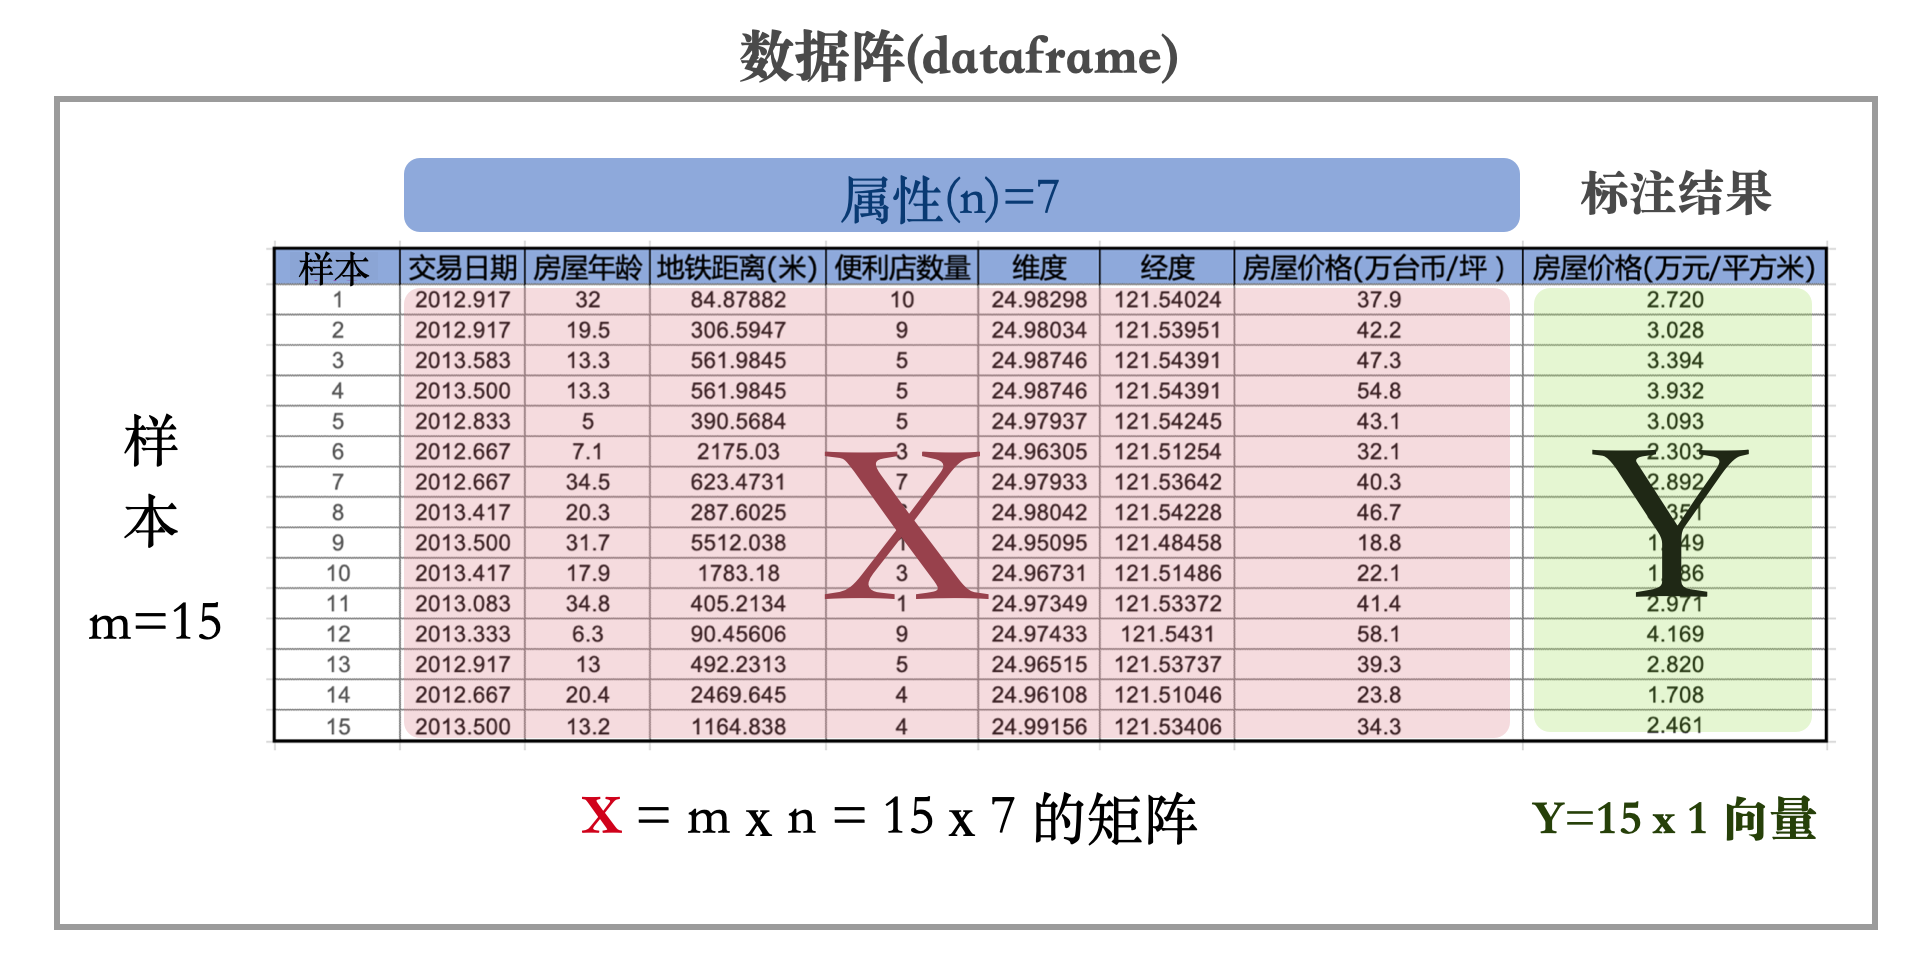
\includegraphics[width=0.9\textwidth]{/Users/Michael/Documents/MDLforBeginners/Chapter2/Lecture_slides/fig/dataframeVis.png}
	\caption{数据阵可视化}
\end{figure}
下面我们就来学习\texttt{Python}语言环境下的数据阵操作。按照惯例我们首先加载具体的工具包。有些工具包是辅助我们实验的,有些被标记\texttt{重点内容}的,需要同学们掌握。
\begin{python}
# 加载常用工具包,SenseStudy 目前测试可以加载下列工具包
# 注意,非重点内容不需要掌握
import numpy as np  #重点内容
import pandas as pd  #重点内容
import matplotlib.pyplot as plt  #重点内容
import seaborn as sns
from sklearn import datasets
from sklearn import preprocessing
from sklearn.model_selection import train_test_split
from sklearn.linear_model import Perceptron
\end{python}

\subsection{鸢尾花数据阵构造和读取}

在Python语言中,对数据阵的处理依赖于`pandas`工具包, 本次练习同学们需要重点掌握:
\begin{itemize}
	\item 创作数据阵的方法
	\item 查看数据阵的基本结构,比如维数,属性名称
	\item 调取数据阵中某一行或某一列的方法
\end{itemize}

数据阵的构造的代码为: \hlc{pd.DataFrame(X, index=[ ], columns = [ ])}, 其中$X$是二维的矩阵,包含我们的数据,这里特别提醒同学们,即使$X$只有一行,比如$[1, 2, 3]$,输入的时候也需要放在二维数组里,应该是$[[1, 2, 3]]$。其中\hlc{columns}指的是我们的属性名称,\hlc{index}指的是我们的样本的个数。

\begin{python}
# 创建数据阵的方法,注意list必须是二维
df_a = pd.DataFrame([[1, 2, 3]], columns=['属性1', '属性2', '属性3']) 
print(df_a.head())  # 查看数据阵的前几行
# 例2
df_b = pd.DataFrame([[1, 2, 3], [4, 5, 6]], columns=['name', 'year', 'month'])
df_b.head()
print(df_b.shape)  # 查看维数
\end{python}

现在我们随意创造一个数据阵,来练习对其内容的读取和修改。我们在对数据阵进行修改时,最主要的读取和修改为:
\begin{itemize}
	\item 修改属性名称 
	\item 调取某一行 
	\item 调取某一列 
	\item 修改某一行、某一列或者某一个具体的数据 
\end{itemize}

那么应用到的指令依次为:
\begin{itemize}
	\item \hlc{dataframe.columns}
	\item \hlc{dataframe.iloc[row, :]}
	\item \hlc{dataframe.iloc[:, column]}
	\item \hlc{dataframe.iloc[row, column]}
\end{itemize}
那接下来我们就具体学习一下。

\begin{python}
# 创造一个比较大的数据阵
matrix_A = np.ones([100, 5])  # 100 乘以 5 的全1矩阵
print(matrix_A[:6, :])  # 查看前六行
df_c = pd.DataFrame(matrix_A, columns=['身高(cm)', '体重(kg)', '睡眠(小时)', '卡路里(焦耳)', 'BMI指示'])
print(df_c.head())
print(df_c.columns)
print(df_c.shape)
df_c.rename(columns={'卡路里(焦耳)': '热量(焦耳)'}, inplace=True)  # 修改具体的属性名称
print(df_c.columns)
df_c.columns = ['height(cm)', 'weight(kg)', '睡眠(小时)', 'calorie(焦耳)', 'BMI指示']  # 也可以一次性部分或全部修改
print(df_c.columns)
print(df_c.head())

# 调取和修改某一行
print(df_c.iloc[6, :])  # 第5行
df_c.iloc[1, :] = [1, 2, 3, 4, 5]  # 修改 第二行
print(df_c.head())

# 调取和修改某一列
print(df_c.iloc[:, 2])  # 第三列
df_c.iloc[:, 2] = np.ones([100, 1])*56
print(df_c.head())

# 修改某一数据
df_c.iloc[0, 1] = 176
print(df_c.head())
\end{python}

了解了数据阵在\hlc{Python}中的基本指令后,我们来看一下本章的案例、\texttt{鸢尾花数据集}。

\begin{python}
iris = datasets.load_iris()  # 加载数据阵
print(iris.data[0: 5])
print(iris.target[0:5])
print(iris.feature_names) 
iris.feature_names.append('Category')
iris_df = pd.DataFrame(np.column_stack((iris.data, iris.target)),
                       columns=iris.feature_names)  # 重点内容
iris_df.Category = iris_df.Category.astype(int)
print(iris_df.shape)  # 150 x 5 dataframe, 特征变量矩阵X 为 150 x 4, 即150 个样本, 4个属性, 还有1个结果向量
print(iris_df.head())  # 查看下前5行
\end{python}


\subsection{鸢尾花数据阵可视化}

接下来,我们把鸢尾花数据阵进行可视化,大体看一下的分布形态。具体到\hlc{Python}可视化的内容,我们会在\underline{后面章节中逐步讲解},这里只做演示。
\begin{python}
sns.set(style="whitegrid")  
fig, axes = plt.subplots(1, 2, figsize=(12, 6))
sns.scatterplot(x=iris_df.iloc[:, 0],
                y=iris_df.iloc[:, 1],
                hue=iris_df.iloc[:, 4],
                ax=axes[0], s=80, palette="Set1")
sns.scatterplot(x=iris_df.iloc[:, 2],
                y=iris_df.iloc[:, 3],
                hue=iris_df.iloc[:, 4],
                ax=axes[1], s=80, palette="Set1")
\end{python}


\subsection{鸢尾花种类选取}

现在我们选取两种鸢尾花,并且只对其花瓣的长度和宽度进行可视化。
\begin{python}
iris_df_binary = iris_df[iris_df.Category != 1]  # 选取种类标记为 0 和 2 的鸢尾花
print(iris_df_binary.shape)  # 查看新的维数
print(iris_df_binary.columns)  # 查看属性名称
sns.scatterplot(x=iris_df_binary.iloc[:, 2],
                y=iris_df_binary.iloc[:, 3],
                hue=iris_df_binary.iloc[:, 4],
                s=80, palette="Set1")  # 只对两种鸢尾花进行可视化
\end{python}

通过可视化,我们大体了解了鸢尾花其属性的分布,那么我们来学习下向量的运算,从而帮助我们进行分类。

\subsection{向量的运算和其性质}

因为本章学习需要用到简单的向量运算,所以我们先熟悉下基本的向量运算。向量概念在不同学科中都有使用,在我们人工智能领域,我们通过数学和计算机领域来引入这个概念。在数学中,最初是为了帮助我们解方程组透过矩阵而引入的。我们在本次实验中,会学习:
\begin{itemize}
	\item 向量的加法
	\item 向量的乘法
	\item 向量的点积
\end{itemize}
向量在\hlc{Python}中的表现形式是\hlc{array},所有每当我们要建立一个向量时,我们需要使用下面的代码:
\begin{python}
v1 = np.array([1, 2, 3])  # 建立一个向量
v2 = np.array([3, 4, 5])  # 建立第二个向量
print(v1+v2)  # 向量相加
print(3*v1)  # 向量乘法
v3 = np.dot(v1, v2)  # 向量的点积
print(v3)
\end{python}
注意,向量的点积只能在相同长度的向量之间运行,比如下面的运行会\textbf{报错}。
\begin{python}
v4 = np.array([4, 9, 10, 11])
np.dot(v1, v3)  # raise ValueError, 报错
\end{python}

在课堂中,我们利用下面这张图片讲解了向量运行的几何性质。
\begin{figure}[H]
	\centering
	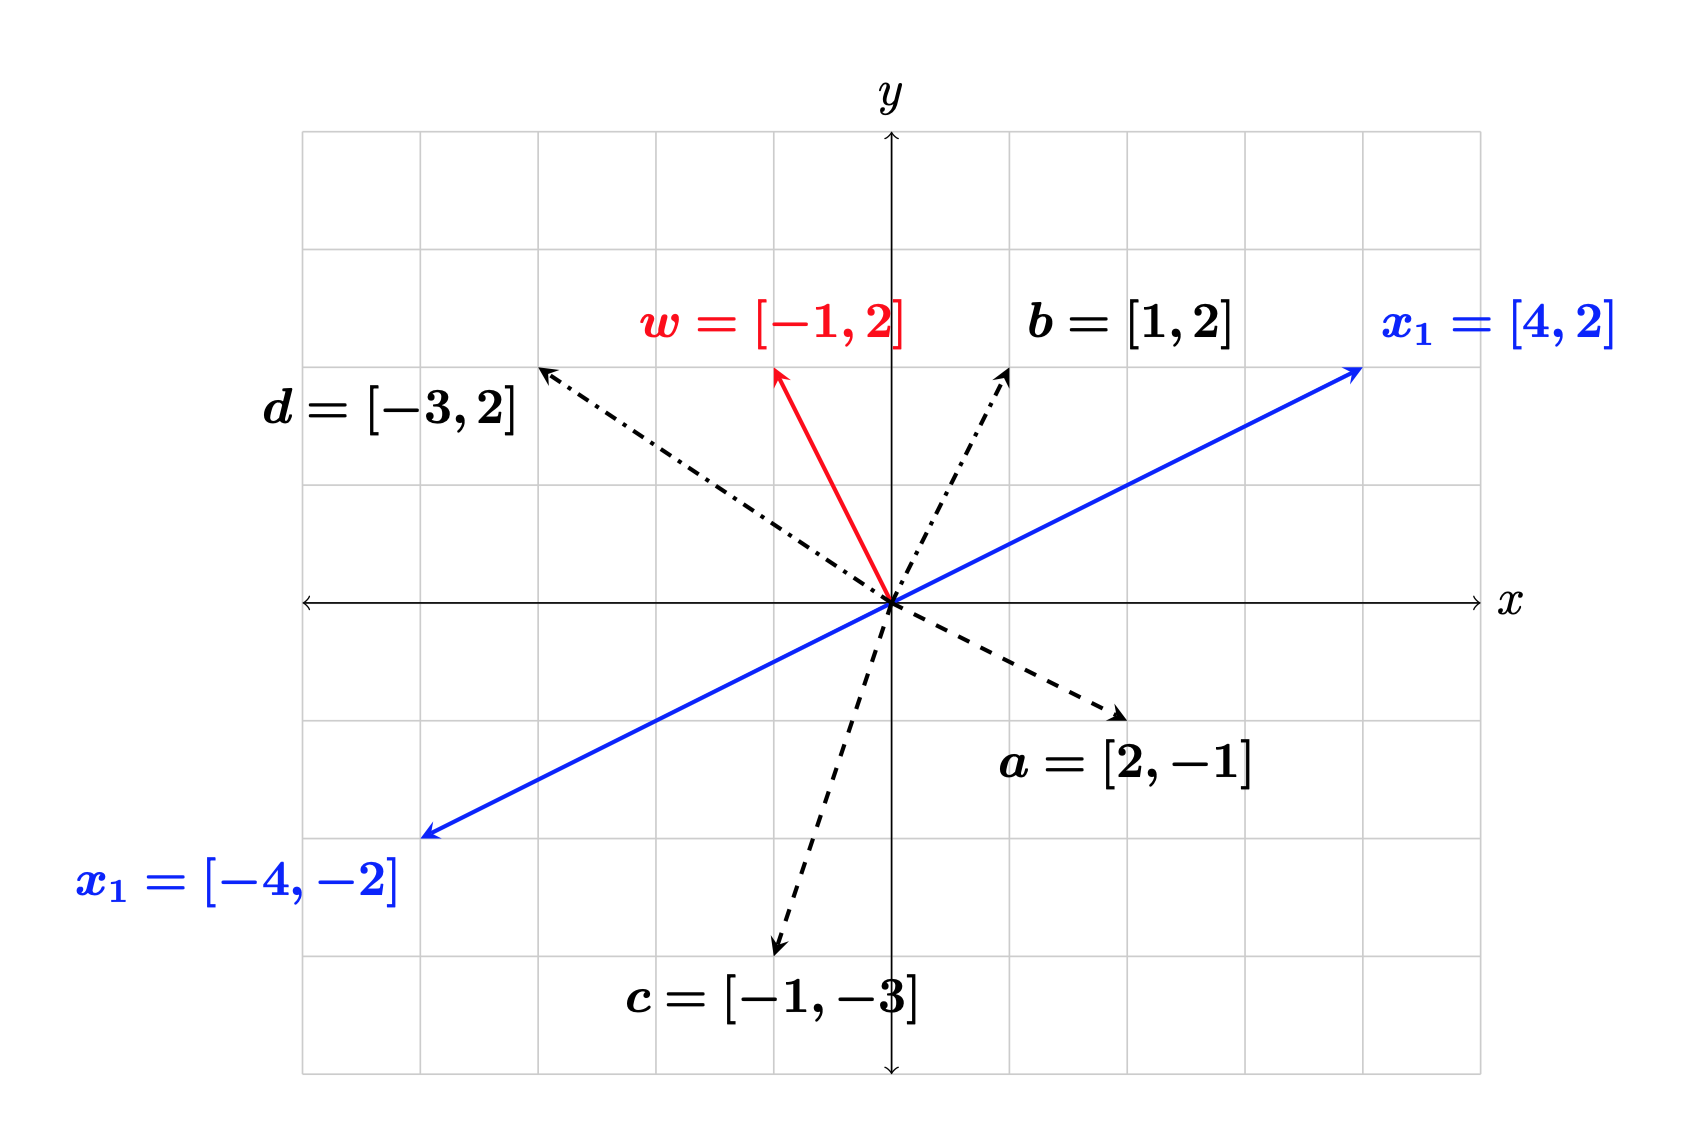
\includegraphics[width=0.9\textwidth]{/Users/Michael/Documents/MDLforBeginners/Chapter2/Lecture_slides/fig/C2C2dotprodt.png}
\end{figure}
那么现在我们就用\hlc{Python}来具体算一下。
\begin{python}
a = np.array([2, -1])
b = np.array([1, 2])
c = np.array([2, -1])
d = np.array([-3, 2])
w = np.array([-1, 2])
print(np.dot(a, w))
print(np.dot(c, w))
print(np.dot(b, w))
print(np.dot(d, w))
x1 = np.array([4, 2])
x2 = np.array([-4, -2])
print(np.dot(x1, w))
print(np.dot(x2, w))
\end{python}
通过上面的运算,我们可以发现点积有很好的几何性质,这个几何性质可以表达为:
\begin{align*}
W \cdot X &= ||W|| ||X|| \cos \theta  \begin{cases}
		> 0 &  0 \leq \theta < \pi/2 \\
		= 0 & \theta = \pi/2  \ \ \text{即$W$与$X$垂直} \\
		< 0 &  \pi 2 < \theta \leq \pi 
	\end{cases}
\end{align*}

下面我们继续通过\hlc{Python}来熟悉向量运算,及其几何性质。整个感知器线性分类和支持向量机的分类原理,都可以用上面这张图来概括。


\section*{实验2: 线性分类和梯度下降法}



\section*{实验2感知器线性二元分类和支持向量机}









\end{document}